
\section*{Introduction}
[Explain brightly what the report is about.]

\section*{Method}
The implementation utilized standard C libraries, including \texttt{stdlib.h}, \texttt{stdio.h}, \texttt{time.h}, and \texttt{limits.h}. Measurements were conducted on an Intel i7-13700K CPU with default frequency settings. The code was compiled using GCC without optimizations (\texttt{-O0}). Code from previous labs was used to conduct the benchmark. The benchmark methodology includes random generation of array elements, 50 iterations to obtain reliable average measurements, and time measurements in nanoseconds using \texttt{clock\_gettime()}. Internet tool "mycurvefit.com" have been used to find the best fit function for the data.

\section*{Hypothesis}
In the normal and inproved implementation of queue, the time of enque and dequeue a specific length of elements in a array will be recorded.
Since the normal inplementation do we need to go through the whole array till the end to enque, there fore the time complextiy will be $O(n)$.
In the improved implementation, we will use a pointer to point to the end of the queue to be enque, so the time complexity will be $O(1)$.
And since both implementations will perfrom dequeue by removing the first node of the queue, and let the second node become the first node. And the solution for the inplementation stays the same. There fore the time complexity for dequeue operations will be $O(1)$ for both implementations.


\section*{Code Review}
In this paragraph, some inportant code snippets will be shown and explained.
\subsection*{empty}
\begin{minted}{c}
int empty(queue *q) {
    return (q->first == NULL);
}
\end{minted}
The code above shows the empty function of the queue. The function will return 1 if the queue is empty, and 0 if the queue is not empty. The time complexity of this function is $O(1)$.

\subsection*{dequeue}
\begin{minted}{c}
int dequeue(queue *q) {
    int res = 0;
    if (q->first != NULL) {
        node *nd = q->first;
        res = nd->value;
        q->first = nd->next;
        free(nd);
    }
    return res;
}
\end{minted}
The code above shows the dequeue function of the queue. The function will return the value of the first node of the queue, and remove the first node of the queue. And let the second node become the first node of the queue. The time complexity of this function is $O(1)$.

\subsection*{Enque- Normal Implementation}
\begin{minted}{c}
void enque(queue* q, int v) {
    node *nd = (node*)malloc(sizeof(node));
    nd->value = v;
    nd->next = NULL;

    node *nxt = q->first;
    if (nxt == NULL) {
        q->first = nd;
        return;
    }
    while (nxt->next != NULL) {
        nxt = nxt->next;
    }
    nxt->next = nd;
}
\end{minted}
The code above shows the normal implementation of the enque function. In this implementation, we need to go through the whole queue to find the last node of the queue. And this makes the time complexity of the enque function to be $O(n)$.

\subsection*{Enque- Inproved Implementation}
\begin{minted}{c}
void enque(queue* q, int v) {
    node *nd = (node*)malloc(sizeof(node));
    nd->value = v;
    nd->next = NULL;

    
    if (q->first == NULL) {
        q->first = nd;
        q->last = nd;
        return;
    }
    q->last->next = nd;
    q->last = nd;
}
\end{minted}
To achive the goal of inserting a node directly on the last node, we need to create a new last node in the queue structure. And we will use this last node to point to the last node of the queue. And in the enque function, we will use this last node to point to the new node to be enque. And this make the time complexity be become $O(1)$.

\section*{Results and Analysis}
\subsection*{Normal queue implementation}
\begin{table}[h]
    \centering
    \begin{tabular}{|l|c|c|c|c|}
    \hline
    \textbf{Size} & \textbf{Min (µs)} & \textbf{Max (µs)} & \textbf{Avg (µs)} & \textbf{Avg/op (ns)} \\
    \hline
    1000 & 490.28 & 2410.69 & 845.58 & 845.58 \\
    2000 & 1973.71 & 2330.07 & 2042.42 & 1021.21 \\
    4000 & 7877.75 & 9944.86 & 8174.96 & 2043.74 \\
    8000 & 30707.86 & 34803.72 & 31376.74 & 3922.09 \\
    16000 & 122342.77 & 132523.96 & 123654.04 & 7728.38 \\
    32000 & 485247.17 & 496878.95 & 487832.40 & 15244.76 \\
    64000 & 1947782.08 & 1995377.47 & 1952189.52 & 30502.96 \\
    \hline
    \end{tabular}
    \caption{Performance of Normal Queue implementation}
    \label{tab:queue_perf}
\end{table}
Here above is the performance of the normal queue implementation. As we can see from the table, with random generated elements, the time complexity follows a linear growth with the size of the queue. Which fit to our hypothesis that the time complexity of the enque function is $O(n)$.


\subsection*{Inproved queue implementation}
\begin{table}[h]
    \centering
    \begin{tabular}{|l|c|c|c|c|}
    \hline
    \textbf{Size} & \textbf{Min (µs)} & \textbf{Max (µs)} & \textbf{Avg (µs)} & \textbf{Avg/op (ns)} \\
    \hline
    1000 & 54.24 & 102.56 & 58.75 & 58.75 \\
    2000 & 22.61 & 157.66 & 40.42 & 20.21 \\
    4000 & 44.92 & 70.79 & 47.62 & 11.91 \\
    8000 & 89.62 & 155.09 & 95.12 & 11.89 \\
    16000 & 182.24 & 273.46 & 202.08 & 12.63 \\
    32000 & 502.77 & 582.42 & 517.86 & 16.18 \\
    64000 & 791.99 & 1170.50 & 1043.34 & 16.30 \\
    128000 & 1589.10 & 2197.81 & 2075.89 & 16.22 \\
    \hline
    \end{tabular}
    \caption{Performance of Improved Queue implementation}
    \label{tab:improved_queue_perf}
\end{table}
Here above is the performance of the improved queue implementation. As we can see from the table, with random generated elements, the time complexity follows a constant growth with the size of the queue. Which fit to our hypothesis that the time complexity of the enque function is $O(1)$.

\subsection*{Analysis}
\begin{figure}[h]
    \centering
    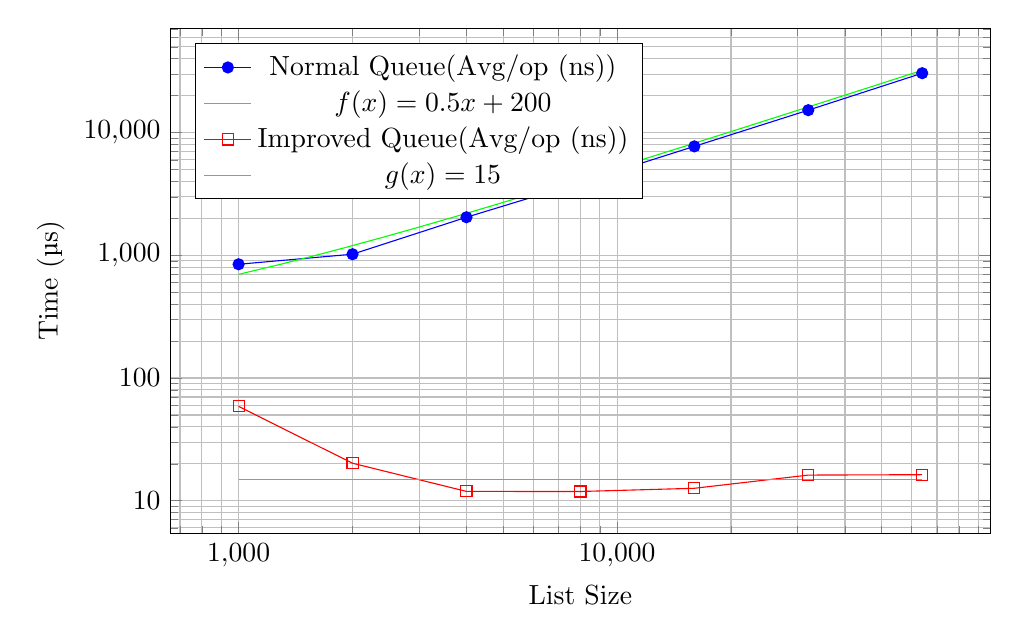
\begin{tikzpicture}
    \begin{axis}[
    xlabel={List Size},
    ylabel={Time (µs)},
    width=12cm,
    height=8cm,
    xmode=log,
    ymode=log,
    grid=both,
    legend pos=north west,
    log ticks with fixed point
    ]
    % Normal Queue
    \addplot[blue, mark=*] coordinates {
        (1000, 845.58)
        (2000, 1021.21)
        (4000, 2043.74)
        (8000, 3922.09)
        (16000, 7728.38)
        (32000, 15244.76)
        (64000, 30502.96)
    };
    \addlegendentry{Normal Queue(Avg/op (ns))}

    \addplot[color=green, domain=1000:64000, samples=20] {x/2 + 200};
    \addlegendentry{$f(x) = 0.5x + 200$}

    % Improved Queue
    \addplot[red, mark=square] coordinates {
        (1000, 58.75)
        (2000, 20.21)
        (4000, 11.91)
        (8000, 11.89)
        (16000, 12.63)
        (32000, 16.18)
        (64000, 16.30)
    };
    \addlegendentry{Improved Queue(Avg/op (ns))}
    
    \addplot[color=green, domain=1000:64000, samples=20] {15};
    \addlegendentry{$g(x) = 15$}

    \end{axis}
    \end{tikzpicture}
    \caption{Log-log plot comparing Normal Queue vs Improved Queue performance (Avg/op)}
    \label{fig:queue_comparison}
\end{figure}
From this figure we can see a clear difference between the normal queue implementation and the improved queue implementation. The normal queue implementation has a linear growth with the size of the queue, while the improved queue implementation has a constant growth with the size of the queue. This fits to our hypothesis that the time complexity of the enque function in the normal queue implementation is $O(n)$, and the time complexity of the enque function in the improved queue implementation is $O(1)$.
I also found the best fit function for the data. And the best fit function for the normal queue implementation is $f(x) = 0.5x + 200$, and the best fit function for the improved queue implementation is $g(x) = 15$.


\section*{Conclusion}
 [Summerize the report and the results. Explain what we have learned from the report. And what we can do to improve the performance of the queue implementation.
 Write in plain text without any points.
 ]

\end{document}
